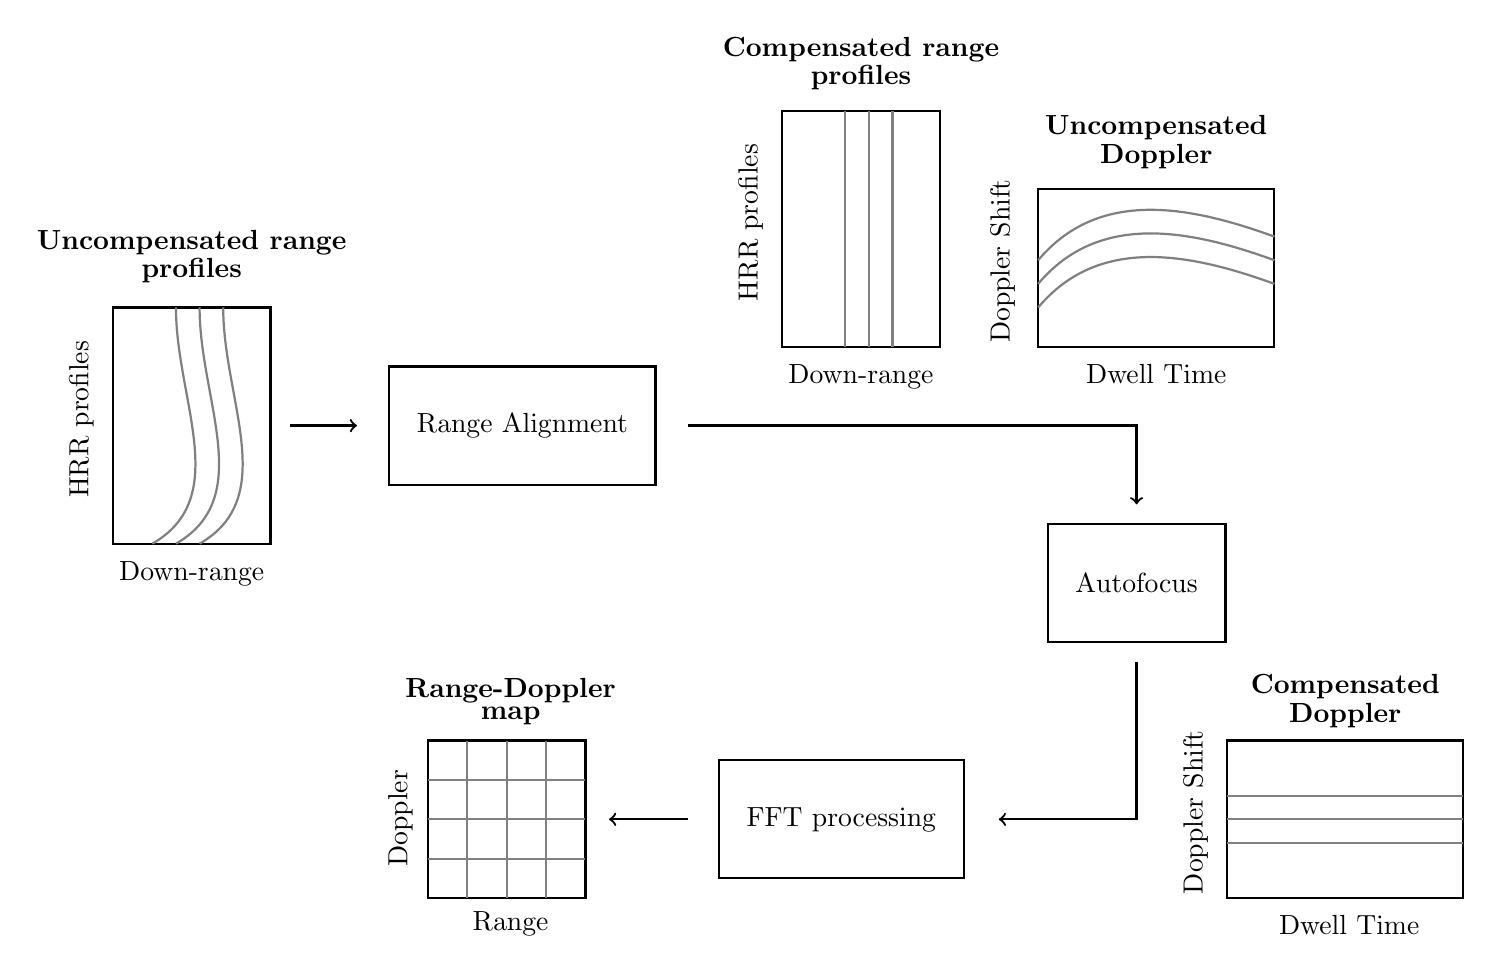
\begin{tikzpicture}
    % Draw the uncompensated range block with curved lines
    \draw[thick] (0,0) rectangle (2,3);
    \draw[thick, gray] (0.5,0) to[out=30, in=270] (0.8,3);
    \draw[thick, gray] (0.8,0) to[out=30, in=270] (1.1,3);
    \draw[thick, gray] (1.1,0) to[out=30, in=270] (1.4,3);
    % Label the axes 
    \node[below=0.8cm] at (1,0.7) {Down-range};
    \node[left=0.8cm,rotate=90] at (0.4,2.7) {HRR profiles};
    \node[above=0.5cm,font=\bfseries] at (1,3.05) {Uncompensated range} node[below,font=\bfseries] at (1,3.75) {profiles};

    % Add an arrow pointing to the right
    \draw[->, thick] (2.25,1.5) -- (3.1,1.5);

    % Draw the Range Alignment block
    \node[draw, thick, rectangle, minimum width=2cm, minimum height=1.5cm, inner sep=10pt] at (5.2,1.5) {Range Alignment};
    
    % Draw the compensated range block with straight lines
    \draw[thick] (8.5,2.5) rectangle (10.5,5.5);
    \draw[thick, gray] (9.3,2.5) -- (9.3,5.5);
    \draw[thick, gray] (9.6,2.5) -- (9.6,5.5);
    \draw[thick, gray] (9.9,2.5) -- (9.9,5.5);
    % Label the axes 
    \node[below=0.8cm] at (9.5,3.2) {Down-range};
    \node[left=0.8cm,rotate=90] at (8.9,5.2) {HRR profiles};
    \node[above=0.5cm,font=\bfseries] at (9.5,5.5) {Compensated range} node[below,font=\bfseries] at (9.5,6.2) {profiles};

    % Draw the uncompensated Doppler block with straight lines
    \draw[thick] (11.75,2.5) rectangle (14.75,4.5);
    \draw[thick, gray] (11.75, 3) to[out=50, in=-200] (14.75, 3.3);
    \draw[thick, gray] (11.75,3.3) to[out=50, in=-200] (14.75,3.6);
    \draw[thick, gray] (11.75,3.6) to[out=50, in=-200] (14.75,3.9);
    % Label the axes 
    \node[below=0.8cm] at (13.25,3.2) {Dwell Time};
    \node[left=0.8cm,rotate=90] at (12.1,4.75) {Doppler Shift};
    \node[above=0.5cm,font=\bfseries] at (13.25,4.5) {Uncompensated} node[below,font=\bfseries] at (13.25,5.2) {Doppler};
    
    % Add an arrow pointing to the right
    \draw[->, thick] (7.3,1.5) -- (13,1.5)--(13,0.5);
    
    % Draw the Autofocus block
    \node[draw, thick, rectangle, minimum width=2cm, minimum height=1.5cm, inner sep=10pt] at (13,-0.5) {Autofocus};

     % Add an arrow pointing down
    \draw[->, thick] (13,-1.5)--(13,-3.5)--(11.25,-3.5);

    % Draw the compensated Doppler block with straight lines
    \draw[thick] (14.15,-2.5) rectangle (17.15,-4.5);
    \draw[thick, gray] (14.15, -3.2) -- (17.15, -3.2);
    \draw[thick, gray] (14.15,-3.5) -- (17.15,-3.5);
    \draw[thick, gray] (14.15,-3.8) -- (17.15,-3.8);
    % Label the axes 
    \node[below=0.8cm] at (15.7,-3.8) {Dwell Time};
    \node[left=0.8cm,rotate=90] at (14.55,-2.25) {Doppler Shift};
    \node[above=0.5cm,font=\bfseries] at (15.65,-2.6) {Compensated} node[below,font=\bfseries] at (15.65,-1.9) {Doppler};


    % Draw the FTT block
    \node[draw, thick, rectangle, minimum width=2cm, minimum height=1.5cm, inner sep=10pt] at (9.25,-3.5) {FFT processing};

     % Add an arrow pointing left
    \draw[<-, thick] (6.3,-3.5)--(7.3,-3.5);

    % Range-Doppler map
    \draw[thick] (4,-2.5) rectangle (6,-4.5);
    \draw[thick, gray] (4, -3) -- (6, -3);
    \draw[thick, gray] (4,-3.5) -- (6,-3.5);
    \draw[thick, gray] (4,-4) -- (6,-4);
    \draw[thick, gray] (4.5, -2.5) -- (4.5, -4.5);
    \draw[thick, gray] (5, -2.5) -- (5, -4.5);
    \draw[thick, gray] (5.5, -2.5) -- (5.5, -4.5);
    % Label the axes 
    \node[below=0.8cm] at (5.05,-3.75) {Range};
    \node[left=0.8cm,rotate=90] at (4.45,-2.75) {Doppler};
    \node[above=0.5cm,font=\bfseries] at (5.05,-2.65) {Range-Doppler} node[below,font=\bfseries] at (5.05,-1.95) {map};
\end{tikzpicture}